\chapter{Giải thuật Deep Sort theo dõi từng người trong khung hình}
Qua các chương trước, luận văn đã trình bày thuật toán, lý thuyết cũng nhhư cách thức hoạt động của chương trình nhận dạng ngôn ngữ ký hiệu. Ở chương này, luận văn sẽ trình bày giải thuật Deep Sort dùng để theo dõi từng người trong khung hình, đánh số thứ tự từng người, cùng với ngôn ngữ ký hiệu của họ muốn diễn đạt.

Phát hiện đối tượng và theo dõi đối tượng là một trong những chủ đề được thị giác máy tính nghiên cứu từ rất lâu. Các thành tựu của chúng đã đạt đến những thành công rất cao cũng như được ứng dụng rộng rãi vào đời sống. Phát hiện đối tượng (objects detection) chỉ tập trung vào việc phát hiện từng đối tượng, đặt chúng trong từng khung hình riêng lẻ và sau đó phân loại đối tượng đó. Việc phát hiện đối tượng chỉ dừng lại ở đây, như vậy đối với cùng một đối tượng nhưng với các khung hình liên tiếp nhau, máy tính sẽ không thể biết được 2 khung hình này chứa cùng một đối tượng . Khác với các thuật toán phát hiện đối tượng, các thuật toán theo dõi đối tượng đều hoạt động theo cách thức khóa từng đối tượng trong khung hình, xác định duy nhất từng đối tượng và theo dõi tất cả chúng cho đến khi chúng rời khỏi khung hình. Ví dụ, nếu máy tính phát hiện được 3 ôtô trong một khung hình, trình theo dõi sẽ phải xác định được 3 đối tượng riêng biệt, đánh số thứ tự chúng và theo dõi qua các khung hình tiếp theo. Theo dõi đối tượng bao gồm theo dõi đối tượng đơn(single object tracking) và theo dõi đa đối tượng (multiple object tracking). Trong phần này, luận văn sẽ chủ yếu đề cập đến các thuật toán theo dõi đa đối tượng cụ thể là giải thuật Deep Sort (được ứng dụng trong luận văn).  

\section{Lý thuyết thuật toán}
Phổ biến nhất và là một trong những thuật toán đơn giản nhất để theo dõi là Deep Sort (Simple Online and Realtime Tracking \cite{wojke2017simple}). Thuật toán này có thể theo dõi nhiều đối tượng trong thời gian thực nhưng thuật toán chỉ liên kết các đối tượng đã phát hiện trên các khung khác nhau dựa trên tọa độ của kết quả phát hiện, như hình \ref{fig:sort}.

\FloatBarrier
\begin{figure}[htp]
\begin{center}
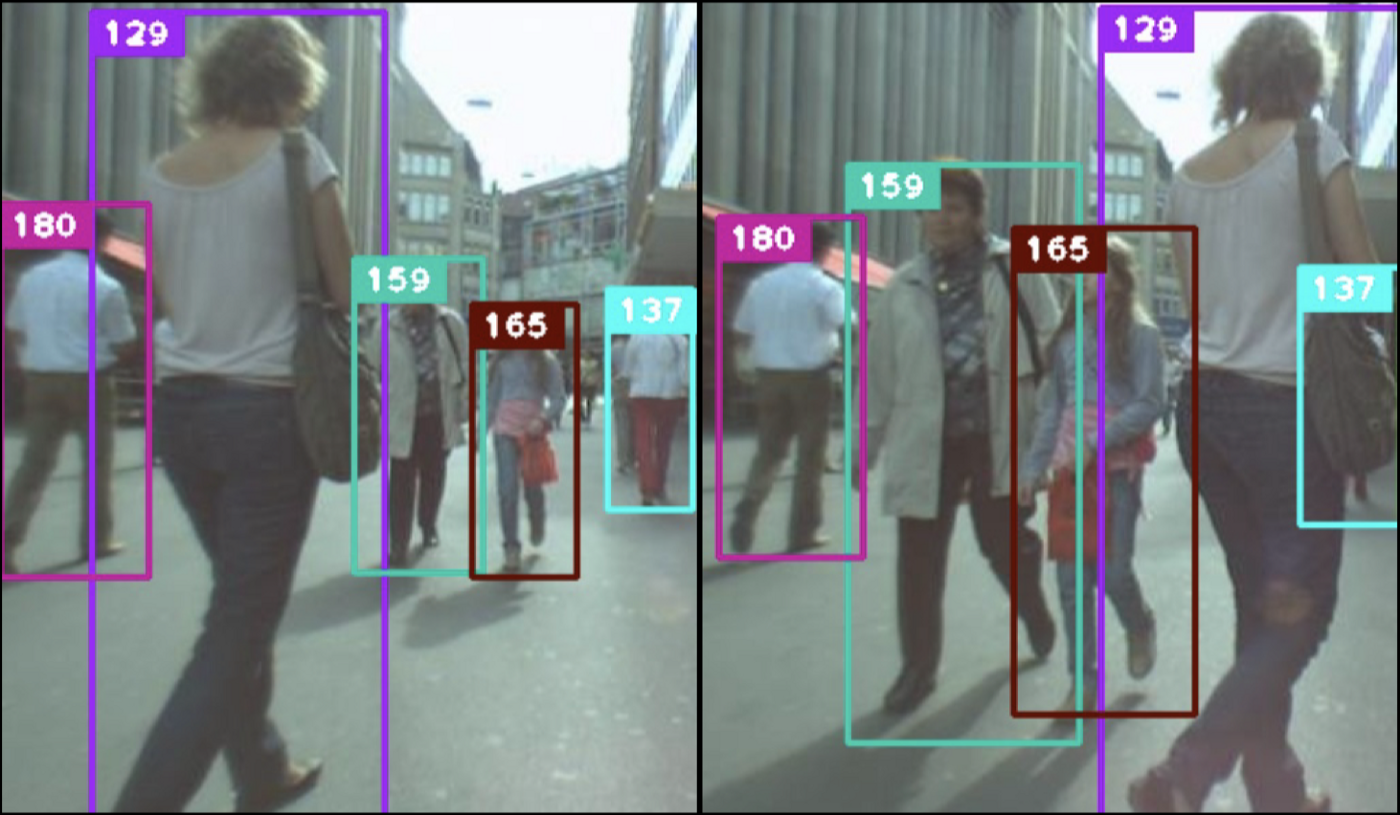
\includegraphics[scale=0.3]{chap5/c5_figs/sort.png}
\end{center}
\caption{Thuật toán Deep Sort}
\label{fig:sort}
\end{figure}
\FloatBarrier
\centerline{(Nguồn : "Simple Online and Realtime Tracking with a Deep Association Metric" \cite{wojke2017simple})}

Deep Sort dụng một phương pháp lý thuyết theo dõi đơn với bộ lọc Kalman hồi quy và liên kết dữ liệu theo từng frame. Các mục sau sẽ mô tả những thành phần chính của một hệ thống Deep Sort.

\subsection{Xử lý theo dõi và ước tính trạng thái}
Bộ lọc Kalman là một thành phần cốt yếu của Deep SORT. Framework của xử lý theo dõi và bộ lọc Kalman hầu hết giống với công thức ban đầu trong của SORT. Giả sử rằng một trường hợp theo dõi tổng quát, camera không thể điều chỉnh và không có thông tin chuyển động có sẵn. Mặc dù các trường hợp này đặt ra một thách thức đối với framework lọc, đó là thiết lập phổ biến nhất được xem xét trong các nghiên cứu theo dõi nhiều đối tượng gần đây. Do đó, phương pháp theo dõi được định nghĩa bởi một không gian trạng thái 8 chiều $( u, v, \gamma , h,  \dot{x} , \dot{y}, \dot{\gamma}, \dot{h})$ chứa vị trí trung tâm hộp bao quanh $(u, v)$ , tỷ lệ khung hình $\gamma$, chiều cao $h$ và vận tốc tương ứng của chúng trong tọa độ ảnh. Thuật toán sử dụng bộ lọc Kalman tiêu chuẩn với chuyển động vận tốc không đổi và mô hình quan sát tuyến tính, trong đó chúng lấy tọa độ giới hạn
$( u, v, \gamma , h)$ làm quan sát trực tiếp trạng thái của đối tượng.

Với mỗi "track" k, chúng ta đếm số lượng khung hình kể từ liên kết phép đo thành công cuối cùng. Bộ đếm này được tăng lên trong suốt quá trình dự đoán bộ lọc Kalman và đặt lại về 0 khi track được liên kết với phép đo. Các track vượt quá độ tuổi tối đa được xác định trước $A_max$ được coi là đã rời khỏi bối cảnh và bị xóa khỏi bộ theo dõi. Các giả thuyết theo dõi mới được khởi tạo cho mỗi phát hiện không thể liên kết với một track hiện có. Những track mới này được phân loại dự kiến trong ba khung hình đầu tiên. Trong thời gian này, chúng ta mong đợi một liên kết phép đo thành công ở mỗi bước. Các track không được liên kết thành công với phép đo trong ba khung đầu tiên của chúng sẽ bị xóa.

\subsection{Bài toán Assignment}
Một cách thông thường để giải quyết mối liên hệ giữa các trạng thái Kalman dự đoán và các phép đo mới là xây dựng một bài toán assignment có thể được giải quyết bằng thuật toán Hungarian. Trong công thức vấn đề này, chúng ta tích hợp thông tin chuyển động và xuất hiện thông qua sự kết hợp của hai metrics thích hợp.
Để kết hợp thông tin chuyển động, chúng ta sử dụng khoảng cách Mahalanobis (bình phương) giữa các trạng thái Kalman dự đoán và các phép đo mới đến. Khoảng cách Mahalanobis lấy những ước tính trạng thái không chắc chắn bằng cách đo xem có bao nhiêu độ lệch chuẩn ra khỏi vị trí theo dõi trung bình. Hơn nữa, bằng cách sử dụng số liệu này, có thể loại trừ các liên kết không có khả năng bằng cách lấy ngưỡng khoảng cách Mahalanobis với khoảng tin cậy 95\% được tính từ phân phối $X^2$ nghịch đảo.

Mặc dù khoảng cách Mahalanobis là một metric liên kết phù hợp khi chuyển động không chắc chắn thấp, trong công thức bài toán ảnh không gian, phân phối trạng thái dự đoán thu được từ khung lọc Kalman chỉ cung cấp ước tính sơ bộ về vị trí đối tượng. Cụ thể, chuyển động của camera không xác định có thể đưa ra các chuyển vị nhanh trong mặt phẳng hình ảnh, làm cho khoảng cách Mahalanobis trở thành một số liệu khá không xác định để theo dõi qua các lần xuất hiện. Do đó, nhóm tác giả tích hợp một metric thứ hai vào bài toán assignment dùng để đo khoảng cách cosine nhỏ nhất giữa track thứ $i$ và track thứ $j$ trong không gian xuất hiện.
Tóm lại, cả hai số liệu bổ sung cho nhau bằng cách đảm nhiệm các khía cạnh khác nhau của bài toán assignment. Một mặt, khoảng cách Mahalanobis cung cấp thông tin về các vị trí đối tượng có thể dựa trên chuyển động, đặc biệt hữu ích cho các dự đoán ngắn hạn. Mặt khác, khoảng cách cosin xem xét thông tin ngoại hình, đặc biệt hữu ích để phục hồi danh tính sau khi xuất hiện dài hạn.

\subsection{Matching cascade}
Thay vì giải quyết các liên kết đo lường để theo dõi trong một bài toán assignment toàn cục, một cascade giải quyết một loạt các bài toán con được giới thiệu. Khi một đối tượng bị chặn trong một khoảng thời gian dài hơn, các dự đoán bộ lọc Kalman tiếp theo làm tăng độ không chắc chắn liên quan đến vị trí của đối tượng. Do đó, khối xác suất trải ra trong không gian trạng thái và khả năng quan sát trở nên ít đạt đỉnh hơn. Theo trực giác, số liệu liên kết nên tính đến sự chênh lệch khối lượng xác suất này bằng cách tăng khoảng cách đo theo dõi. 
Ngược lại, khi hai track cạnh tranh cho cùng một phát hiện, khoảng cách Mahalanobis tạo ra sự không chắc chắn lớn hơn, bởi vì nó có hiệu quả làm giảm khoảng cách về độ lệch chuẩn của bất kỳ phát hiện nào đối với ý nghĩa của track được quan sát. Đây là một đặc điểm không mong muốn vì nó có thể dẫn đến tăng phân đoạn track và các tracks không ổn định. Do đó, một cascade phù hợp, cái mà ưu tiên cho các đối tượng thường xuyên nhìn thấy hơn, để mã hóa khái niệm về xác suất lan truyền trong khả năng liên kết

\section{Kết quả}

Áp dụng giải thuật Deep Sort, luận văn đã theo dõi và đánh số thứ tự được những người có trong khung hình (\ref{fig:deep_sort}).
\FloatBarrier
\begin{figure}[htp]
\begin{center}
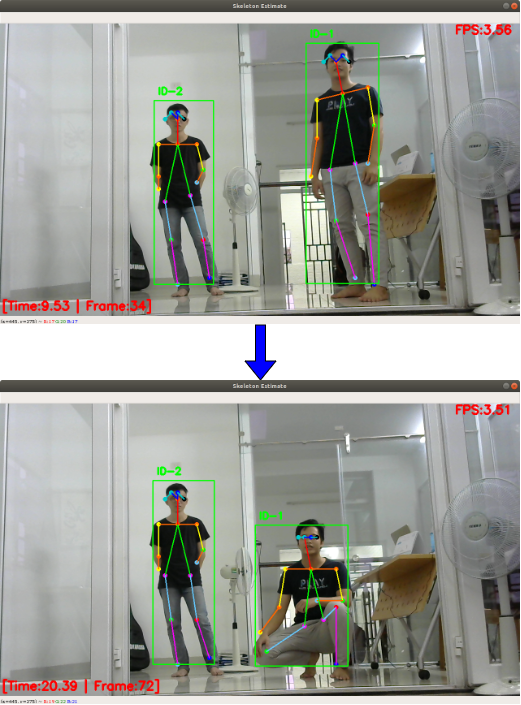
\includegraphics[scale=0.8]{chap5/c5_figs/deep_sort.png}
\end{center}
\caption{Kết quả Deep Sort}
\label{fig:deep_sort}
\end{figure}
\FloatBarrier

Sau khi áp dụng phương pháp này, luận văn nhận thấy thuật toán áp dụng có khả năng theo dõi số lượng lớn người trong khung hình. Tuy nhiên khi có người bị che khuất hoặc người này đi ra sau người kia, thuật toán sẽ theo dõi sai. Phần tiếp theo luận văn sẽ trình bày mô hình thực nghiệm và kết quả cũng như những đánh giá của ứng dụng mà luận văn đã xây dựng.